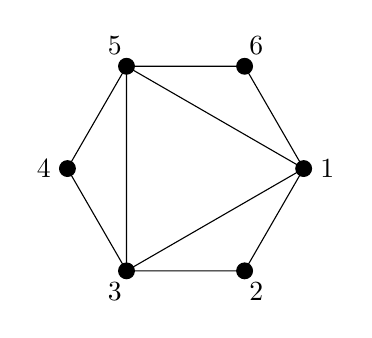
\begin{tikzpicture}
\def \n {1}
\def \R {1.5cm}
\def \RR {1.8cm}
\def \one {0}
\def \two {-60}
\def \three {-120}
\def \four {-180}
\def \five {-240}
\def \six {-300}
\draw (0:\R) \foreach \x in {-60,-120,-180,-240,-300} {
            -- (\x:\R)
        } -- cycle;
\foreach \x in {0,-60,-120,-180,-240,-300} {
        \draw [fill] (\x:\R)  circle [radius=0.1];
        }
\foreach \x/\i in {0/1,-60/2,-120/3,-180/4,-240/5,-300/6} {
        \node at (\x:\RR) {\i};
        }
\draw (\one:\R) -- (\three:\R) -- (\five:\R) --cycle;
\end{tikzpicture}
